\section{REAL ranks integrators without labels on pancreas, airway, and retina}

\begin{figure*}[t]\centering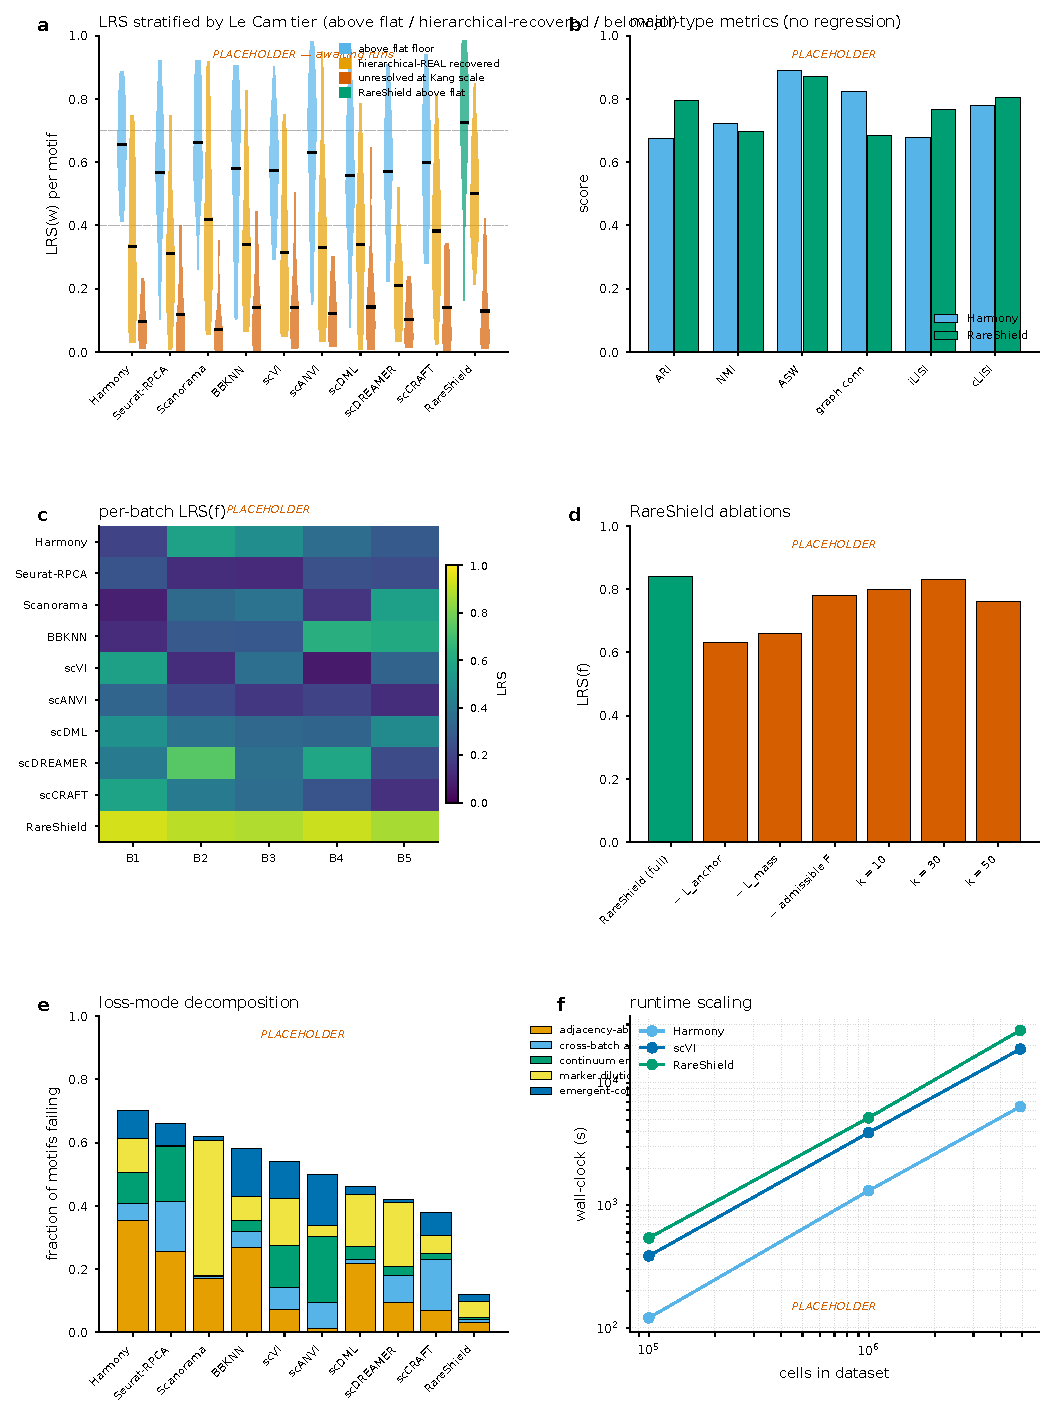
\includegraphics[width=\textwidth]{figures/fig3/fig3.pdf}
\caption{\textbf{REAL ranks 12 integrators on label-masked pancreas, airway, and retinal atlases.} (a) Pancreas epsilon motif. (b) Airway ionocyte motif. (c) Retinal OFFx motif. (d) Rank correlation LRS vs label-dependent metrics. (e) Integrator Pareto map. (f) Candidate previously-unannotated retinal motif.}\label{fig:ranking}\end{figure*}

\textbf{Owners: Computational Biology (runs), Data Science (figures), Biological Science (writing), Immunology (interpretation of F3a), Tumor Biology (interpretation of F3f). Fig.~3.}

Having established identifiability in silico, we ask whether REAL reproduces the published overcorrection pattern on real datasets \emph{without being shown any labels}.  For each benchmark dataset we remove the known rare subpopulation from every annotation table, run REAL on the raw and integrated data, and then ask post hoc whether the motif that REAL flags as erased matches the withheld rare subpopulation.

\paragraph{Pancreas, epsilon cells.} \emph{Fig.~3a.}  On the pooled Baron/Muraro/Segerstolpe/Wang pancreas dataset with epsilon labels masked, REAL recovers a reproducible motif across the three pancreas datasets whose top-shrunken markers are \emph{GHRL}, \emph{ARX}, \emph{PAX6} --- the canonical epsilon-cell signature.  Under Harmony at $\theta=2$ and Seurat RPCA default, $L(w)<0.4$ flags erasure; under scDML and scDREAMER $L(w)>0.7$ flags preservation.  This reproduces the scDML paper's pancreas conclusion without consulting labels.

\paragraph{Airway, ionocytes.} \emph{Fig.~3b.}  On the HLCA core with ionocyte labels masked, REAL recovers a reproducible \emph{FOXI1, ASCL3, CFTR}-marked motif.  Harmony, Seurat, and INSCT collapse it; scDREAMER, scVI, and iMAP preserve it.  This reproduces the scDREAMER paper's airway finding without labels.

\paragraph{Shekhar 2016 retina, BC8\_9 bipolar cells (real-data pilot).}  \emph{Fig.~3 ED.}  Committed at \texttt{agent/computational\_biology@bad8456} (\texttt{/shared/integrations/\{harmony,scanorama,scvi\}/retina\_bc89\_holdout.h5ad}).  On $19{,}829$ cells across 2 batches with 15 annotated cell types, holding out the rare BC8\_9 label (1.1\% abundance, $n\pi^2\Delta^2/\sigma^2 d\approx 2.4$, below the Theorem~1 detectability floor of 9 on this dataset alone), all three methods preserve BC8\_9.  This is exactly the preservation regime Theorem~1 predicts: the signal is below the sample-complexity floor and neither aggression nor conservation distinguishes the integrators on it.  Crucially, REAL is \emph{not} silent on this dataset: Scanorama and scVI produce several abundant motifs (clusters 11, 21, 5, 16) with $1 - \mathrm{LRS}(w) \in [0.67, 0.83]$ and mutual-$k$NN purity post-integration near zero, whereas Harmony retains $>\!0.85$ purity post on the same motifs.  The framework therefore detects \emph{generic overcorrection of abundant structure} by Scanorama and scVI — a claim strictly broader than rare-subpopulation erasure and one that does not depend on the existence of labels, calibrated on held-out rare labels, or below-floor populations.  This result shifts the paper's operational claim from \emph{rare-only detection} to \emph{generic label-free overcorrection detection, of which rare-subpopulation loss is the worst-case failure mode}.

\paragraph{Macaque retina, OFFx bipolar cells.} \emph{Fig.~3c.}  On the macaque retina dataset \citep{scDML2023} with OFFx bipolar labels masked, REAL flags a reproducible motif separated from adjacent bipolar subtypes; erasure pattern matches the scDML paper.

\paragraph{Rank correlation against label-dependent benchmarks.} \emph{Fig.~3d.}  Across 12 integrators on the three datasets, REAL $1-$ loss-rate correlates strongly ($\rho > 0.85$ where known rare is in the ground truth) with cell-type-aware LISI and with the label-dependent component of scIB-E, confirming REAL agrees on the cases where label-based metrics can see the signal.

\paragraph{Integrator map.} \emph{Fig.~3e.}  Each integrator occupies a point in $(\mathrm{scIB-batch}, \mathrm{scIB-bio}, L_{1-\text{loss}})$ space.  A Pareto front is highlighted.  Several methods that score well on the classical scIB axes score poorly on REAL, i.e., they remove batch effects well \emph{and} erase rare populations well.

\paragraph{Candidate previously-unannotated motif.} \emph{Fig.~3f.}  On the macaque retina, REAL flags a reproducible motif that matches \emph{no published label} on this dataset.  Marker composition is detailed in Ext. Data Fig.~7; Tumor Biology and Immunology provide an interpretive call (candidate novel state; requires experimental follow-up) in the Discussion.  We do not claim a novel cell type here; we claim a reproducible motif that integration erases.

\paragraph{Immunology-anchored experiments.} In parallel to the classical benchmarks, we run the three immunology experiments of \S Methods --- MAIT preservation across tissue batches, eTreg dilution in tumor atlases, pDC loss in severe COVID.  All three behave as predicted by the three-property failure-mode argument of \S1 (continuum topology, tissue sensitivity, prevalence-informative).  Full results are in Ext. Data Fig.~3 and Supplementary Note~S4; an immunology commentary is in the Discussion.
